\documentclass[aps,prl,reprint,twocolumns,superscriptaddress]{revtex4-2}
\usepackage[utf8]{inputenc}
\usepackage{amsmath}
\usepackage{amssymb}
\usepackage{txfonts}
\usepackage[hidelinks]{hyperref}
\usepackage{tikz}
\usepackage{hyperref}
\usepackage{color}
\hypersetup{colorlinks=true}
\usepackage{graphicx}
\graphicspath{{figures}}
\usepackage{bm}

\usepackage{chemformula}
\usepackage[capitalise]{cleveref}
\usepackage{siunitx}


\usepackage{tikz}
\usetikzlibrary{external}
\tikzset{external/force remake}
%\tikzexternalize
\newcommand{\deltaq}{\eta_{{\mathrm{min}}}(\theta)/\eta_{{\mathrm{maj}}}(\theta)}

\DeclareMathOperator{\Imm}{Im}
\DeclareMathOperator{\Ree}{Re}
\newcommand{\hc}{\text{h.c.}}
\newcommand{\ii}{\mathrm{i}}
\newcommand{\xx}{\hat{\bm{x}}}
\newcommand{\yy}{\hat{\bm{y}}}
\newcommand{\mdos}{\tilde{m}}
\newcommand{\kF}{k_{F}}
\newcommand{\vs}{v_d}
\newcommand{\FermileveltwoD}{\SI{0.5}{eV}}
\newcommand{\twoDratio}{0.84}
\newcommand{\criticalangle}{\SI{39.9}{\degree}}
\newcommand{\Fermilevel}{\SI{0.5}{eV}}
\newcommand{\mstar}{1.25}
\newcommand{\mzero}{0.4}
\newcommand{\splitting}{\SI{0.6}{eV}}
\newcommand{\muB}{0.025}
\newcommand{\muBShift}{\SI{1.5}{\mu eV}}
\newcommand{\demonenergy}{\SI{2.8}{meV}}
\newcommand{\muBShiftrelative}{0.1}
\newcommand{\muBmax}{0.1}
\newcommand{\pg}[1]{\textcolor{red}{PG: #1}}
\DeclareMathOperator{\sign}{sign}
\newcommand{\subfigref}[2]{Fig.~\hyperref[#1]{\ref*{#1}#2}}
\begin{document}
	\title{Spin demons in $d$-wave altermagnets}
	\date{\today}
	
	\author{Pieter M. Gunnink}
	\email{pgunnink@uni-mainz.de}
	\author{Jairo Sinova}
	\author{Alexander Mook}
	\address{Johannes Gutenberg University Mainz, Staudingerweg 7, Mainz 55128, Germany}
	\begin{abstract}
		Demons are a type of plasmons, which consist of out-of-phase oscillations of electrons in different bands. Here, we show that $d$-wave altermagnets, a recently discovered new class of collinear magnetism, naturally realize a spin demon, which consists of out-of-phase movement of the two spin species.
		The spin demon lives outside of the particle-hole continuum of one of the spin species, and is therefore significantly underdamped, reaching quality factors of $>10$. We show that the spin demon carries a magnetic moment, which inherits the $d$-wave symmetry. Finally, we consider both three and two dimensional $d$-wave altermagnets, and show that spin demons exists in both.
	\end{abstract}
	
	\maketitle
	
	
	\paragraph{Introduction.}
	Altermagnets are a recently discovered class of collinear magnets, characterized by a by a sublattice transposing symmetry involving rotation or mirror operations \cite{smejkalConventionalFerromagnetismAntiferromagnetism2022,smejkalEmergingResearchLandscape2022}. This results in anisotropically spin-split Fermi surfaces, which exhibit a  $d$-wave (or higher even-parity) like order. These spin-split bands can give rise to unusual transport properties \cite{smejkalEmergingResearchLandscape2022,zarzuelaTransportTheorySpintransfer2024,liaoSeparationInverseAltermagnetic2024}, piezomagnetism \cite{aoyamaPiezomagneticPropertiesAltermagnetic2024,yershovFluctuationinducedPiezomagnetismLocal2024}, the generation of spin-splitter torque in
	MRAM geometries \cite{karubeObservationSpinSplitterTorque2022} and chiral split magnon bands \cite{nakaSpinCurrentGeneration2019,liuChiralSplitMagnon2024, smejkalChiralMagnonsAltermagnetic2023}.
	
	The existence of spin-split Fermi surfaces also opens up the possibility of an out-of-phase oscillation of the two spin densities, realizing a \emph{demon}: an acoustic, electrically neutral type of plasmon, first proposed by \textcite{pinesElectronInteractionSolids1956,husainPinesDemonObserved2023}. They are typically gapless, in contrast to the conventional in-phase charge plasmon in three dimensions, and have  been predicted for numerous materials \cite{pinesElectronInteractionSolids1956,ruvaldsAreThereAcoustic1981}, but are typically overdamped due to their overlap with the particle-hole continuum \cite{dassarmaCollectiveModesSpatially1981, sensarmaDynamicScreeningLowenergy2010,agarwalLonglivedSpinPlasmons2014,sadhukhanNovelUndampedGapless2020}. Recent works have however shown that with sufficient separation of the Fermi surfaces, the damping can be suppressed and well-defined quasiparticles are formed \cite{agarwalLonglivedSpinPlasmons2014,husainPinesDemonObserved2023}.
	
	
	In this work, we show that a $d$-wave altermagnetic metal can host a spin-polarized demon, which we dub a \emph{spin demon}. In contrast to the conventional charge plasmon, the spin demon does not live completely outside of the particle-hole continuum, but only outside of the particle-hole continuum of one of the spin species. The spin demon is therefore not completely undamped, but can still reach quality factors of $>10$ for realistic parameters, and is therefore well defined and long lived. We demonstrate the existence of the spin demon in both a three-dimensional (3D) and two-dimensional (2D) $d$-wave altermagnetic metal. We also establish that the spin demon inherits the $d$-wave symmetry of the altermagnetic order parameter, by demonstrating that it has a finite magnetic moment which changes sign as it is rotated through the altermagnetic spin-split plane.
	\begin{figure}
		\tikzsetnextfilename{costheta-current-fig}
		\centering
		%		\begin{tikzpicture}
			%			\node at (-0.5\columnwidth,0) {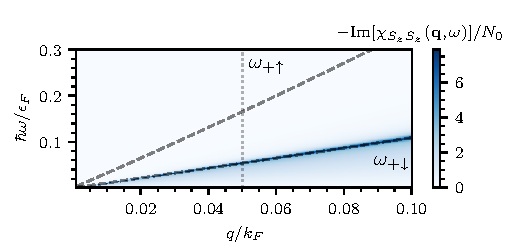
\includegraphics[width=0.5\columnwidth]{SzSz_3D}};
			%			\node at (-0.05\columnwidth,0) {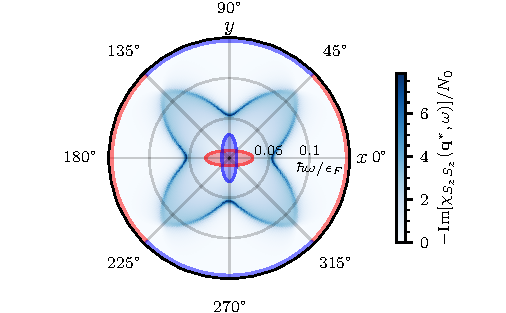
\includegraphics[width=0.35\columnwidth]{polar-plot-chiSzSz}};
			%			%			\node at (-0.5\columnwidth,1.5) {(a)};
			%			\node at (-0.5\columnwidth,-2.8) {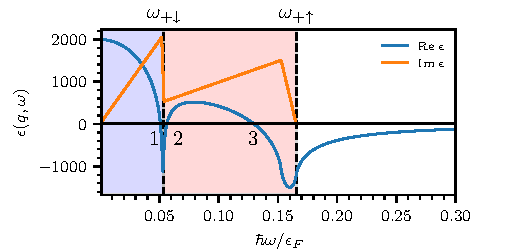
\includegraphics[width=0.5\columnwidth]{linecut-epsilon_3D}};
			%			\node at (-0.05\columnwidth,-2.8) {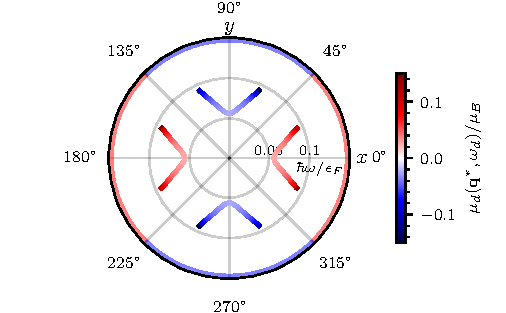
\includegraphics[width=0.35\columnwidth]{polar-plot-sign}};
			%			%			\node at (-0.5\columnwidth,-3.2) {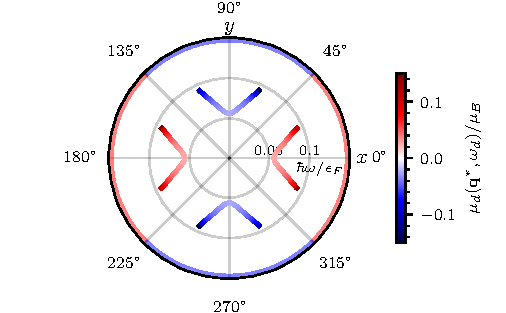
\includegraphics[width=0.5\columnwidth]{			polar-plot-sign}};
			%		\end{tikzpicture}
		%		\begin{tikzpicture}
			%			\node at (-0.5\columnwidth,0) {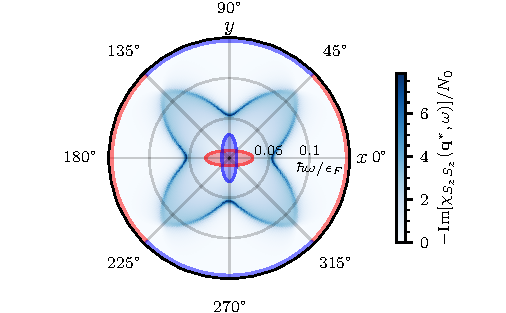
\includegraphics[width=0.5\columnwidth]{polar-plot-chiSzSz}};
			%			\node at (0\columnwidth,0) {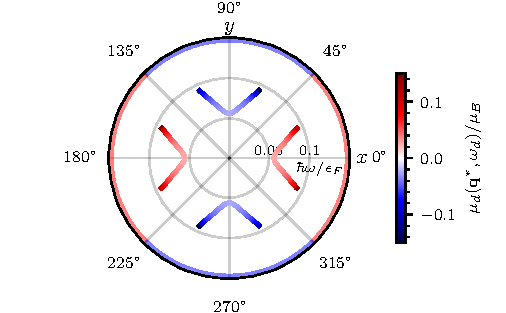
\includegraphics[width=0.5\columnwidth]{polar-plot-sign}};
			%						\node at (-0.5\columnwidth,2) {(a)};
			%						\node at (0.\columnwidth,2) {(b)};
			%		\end{tikzpicture}
		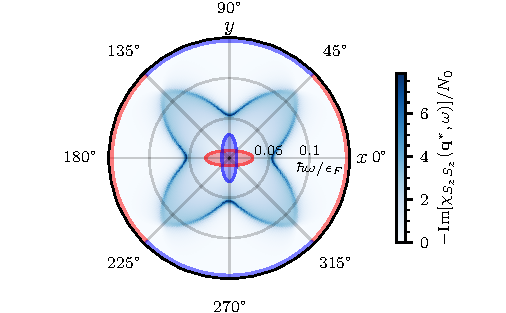
\includegraphics[width=\columnwidth]{polar-plot-chiSzSz}
		\caption{
			The spin–density response function, $\Imm[\chi_{S_zS_z}(\bm q^*,\omega)]$, where $\bm q^*=q\ (\cos\theta,\sin\theta,0)$, rotated in the altermagnetic spin-split plane with a fixed $q=0.05\kF$. The angle indicates $\theta$ and the radial axis the frequency $\omega$. The colors on the ring indicate the projected spin species, with red (blue) spin up (down). The spin demon is the sharp resonance that follows the four-fold rotational symmetry of the $d$-wave altermagnet. The anisotropically spin-split Fermi surfaces are schematically shown at the origin. \label{fig:polar}
			%			(b) The acoustic spin-polarized plasmon frequency for a fixed $q$, rotated in the altermagnetic spin splitting plane with angle $\theta$. The color corresponds to the magnetic moment, showing the $d$-wave character. Along $\bm x,\bm y$, the magnetic moment is $0.05\mu_B$.
		}
	\end{figure}
	
	
	\begin{figure}
		\begin{tikzpicture}
			\node at (-0.5\columnwidth,-3) {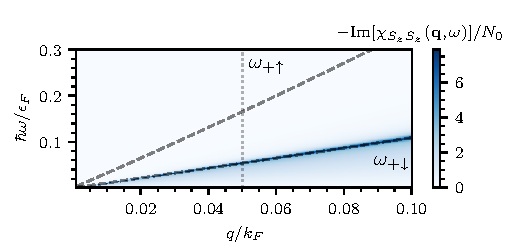
\includegraphics[width=\columnwidth]{SzSz_3D}};
			\node at (-0.5\columnwidth,1) {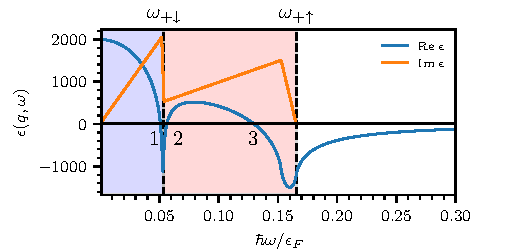
\includegraphics[width=\columnwidth]{linecut-epsilon_3D}};
			\node at (-0.8\columnwidth,3) {(a)};
			\node at (-0.8\columnwidth,-1.4) {(b)};
		\end{tikzpicture}
		\caption{(a) The real and imaginary part of the dielectric function, for $\bm q^* = q \hat{\bm x}$, with $q=0.05\kF$. The zeros of the real part correspond to resonances, the imaginary part determines their damping. The spin demon is the second zero. The blue and red shading indicate where the spin-down and spin-up particle-hole continuum is non-zero. (b)  The spin–spin response function, $\Imm[\chi_{S_zS_z}(\bm q,\omega)]$, for $\bm q\parallel\xx$, showing the existence of a spin demon with a high quality factor. The vertical dotted line corresponds to the $q$ used in (a). In both (a,b), the dashed lines indicate the spin-resolved particle-hole continua edges, $\omega_{\pm-}$.\label{fig:alongx} }
	\end{figure}
	The existence of the spin demon is readily shown by calculating the spin–spin response function, $\Imm[\chi_{S_zS_z}(\bm q,\omega)]$, of an altermagnetic metal, as shown in the altermagnetic spin-split plane in \cref{fig:polar}. The spin demon corresponds to the strongly peaked response in the spin-spin response function, $\Imm[\chi_{S_zS_z}(\bm q,\omega)]$, and follows the four-fold rotational symmetry of the $d$-wave altermagnet, vanishing along the high-symmetry axis, where the electron bands are degenerate. The spin demon is a longitudinal, out-of-phase, oscillation of the spin species, as we will show. In the four different quadrants of the altermagnetic spin-split plane, the majority spin species in this out-of-phase oscillation changes, following the altermagnetic $d$-wave symmetry. 
	
	
	%	 \subfigref{fig:fig1}{(a)}, for $\bm q \parallel \hat x$. The dashed lines indicate the edges of the spin-up and spin-down particle-hole continuum, and the spin demon lives between the two edges of these continua---visible here as a strong peak in $\Imm[\chi_{S_zS_z}]$ just above the edge of the spin-down continuum. 
	
	
	
	
	
	\paragraph{Method.}
	We describe here the spin demon within the random phase approximation (RPA), where the spin-resolved response functions $\chi_{\sigma\sigma'}$ follow \cite{giulianiQuantumTheoryElectron2005}
	\begin{equation}
		\begin{pmatrix}
			\chi_{\uparrow\uparrow} & \chi_{\uparrow\downarrow} \\ 
			\chi_{\downarrow\uparrow} & \chi_{\downarrow\downarrow}
		\end{pmatrix}^{-1} = \begin{pmatrix}
			\chi_\uparrow^{(0)} & 0 \\
			0 & \chi_\downarrow^{(0)}
		\end{pmatrix}
		- v_q \begin{pmatrix}
			1 & 1 & \\ 1 & 1 
		\end{pmatrix} \label{eq:chi-rpa}.
	\end{equation}
	Here, $\chi_\sigma^{(0)}$ is the non-interacting density-density response function for spin $\sigma$ and $v_q=e^2/\epsilon_0 q^2$ is the Fourier transform of the Coulomb interaction. We assume the altermagnet to be oriented such that the spin-splitting is maximal along the $x,y$-axis. The low-energy dispersion of a (planar) $d$-wave altermagnet is then described by \cite{smejkalEmergingResearchLandscape2022}
	\begin{equation}
		\epsilon_{\bm k}^\sigma = \frac{\hbar^2 k^2}{2m_0} + \sigma\frac{\hbar^2 \left( k_x^2-k_y^2\right)}{2m_*} ,
	\end{equation}
	where we take $m_0=\mzero m_e$, $m_*=\mstar m_0$ and a Fermi level of $\epsilon_F=\Fermilevel$. Here, $m_e$ is the electron mass.
	The non-interacting density-density response function can then be found analytically from the Lindhard function \cite{ahnAnisotropicFermionicQuasiparticles2021}; we show details in Secs.~I and II in the Supplemental Material (SM) \footnote{See Supplemental Material at [URL will be inserted by publisher] for a detailed calculation of the spin resolved response functions, details on the numerics, analytical solutions for the spin demon dispersion, quality factor and magnetic moment, and the spin demon in two dimensions and in $g$-wave altermagnets.}. Solving \cref{eq:chi-rpa} for $\chi_{\sigma\sigma'}(\bm q,\omega)$, we find the three response functions $\chi_{nn(\bm q,\omega)},\ \chi_{nS_z}(\bm q,\omega),\ \chi_{S_zS_z}(\bm q,\omega)$ \cite{giulianiQuantumTheoryElectron2005}. We focus here on $\chi_{S_zS_z}(\bm q,\omega)$, which shows the strongest signature of the spin demon:
	\begin{equation}
		\chi_{S_zS_z}(\bm q,\omega)=\frac{\chi_\uparrow^{(0)}+\chi_\downarrow^{(0)}-4v_q\chi_\uparrow^{(0)}\chi_\downarrow^{(0)}}{\epsilon(\bm q,\omega)}
	\end{equation}
	where 
	\begin{equation}
		\epsilon(\bm q,\omega) \equiv 1 - v_q \left(\chi_\uparrow^{(0)}+\chi_\downarrow^{(0)}\right)
	\end{equation}
	is the complex longitudinal dielectric function. We discuss $\chi_{nn}(\bm q,\omega)$ and $\chi_{nS_z}(\bm q,\omega)$ in Sec.~III in the SM. 
	
	Collective modes emerge as the poles of the response function, determined by the zeroes of the longitudinal dielectric function, 
	\begin{equation}
		\epsilon(\bm q,\omega) = 0. \label{eq:poles}
	\end{equation}
	We first analyze the dielectric function in more detail, by showing $\epsilon(\bm q,\omega)$ for a fixed $\bm q\parallel \xx$ in \subfigref{fig:alongx}{(a)}, where we also indicate the spin-polarized particle-hole continua, which edges are given by $\omega_{\sigma+}=\bm v_F^\sigma\cdot \bm q + O(q^2/\kF^2)$, where $\bm v_F^\sigma$ is the spin-dependent Fermi velocity.
	
	We observe the existence of three zeros of the dielectric function. The first and third zero correspond to the spin-down and spin-up acoustic plasmon respectively \cite{kamenevFieldTheoryNonEquilibrium2023}, which are overdamped because they live in their respective particle-hole continuum. The second zero however arises because of the interplay of the spin-up and spin-down particles, and corresponds to the spin demon. Importantly, it sits outside of the spin-down continuum, and therefore the imaginary part of the dielectric function is reduced. This implies that the spin demon is potentially underdamped, which we will show in more detail with the imaginary part of the spin-spin response function, $\Imm[\chi_{S_zS_z}(\bm q,\omega)]$ in \subfigref{fig:alongx}{(b)}. The sharp resonance close the edge of the spin-down continuum is the spin demon, which we observe to be sharply peaked, although it is not completely undamped, due to a finite overlap with the spin-up continuum. We show in Sec.~VII in the SM the spin-spin response function $\Imm[\chi_{S_zS_z}(\bm q,\omega)]$ for a larger range of $q$ values, from which we conclude that for this set of parameters, the spin demon remains well defined for $q/\kF<0.5$.
	
	
	Upon rotation through the altermagnetic spin-split plane, we obtain \cref{fig:polar}, demonstrating that the spin demon is most sharply defined along $x$ and $y$, and vanishes along the nodal lines, where the Fermi surfaces are spin degenerate. 
	The spin demon remains well defined for small tilt angles off the altermagnetic spin-split plane, as shown in Sec.~IV in the SM.
	
	
	
	
	\paragraph{Analysis. }
	In what follows, we constrain $\bm q$ to lie in the altermagnetic spin-split plane, parametrizing $\bm q = q\  (\cos\theta,\sin\theta,0)$. Our analysis is simplified by defining the projected spin splitting of the particle-hole continuum for spin species $\sigma$:
	\begin{equation}
		\eta_{\sigma}(\theta) \equiv \sqrt{\mdos m_0\left( 1+\sigma \frac{m_0}{m_*}\cos2\theta\right)} \label{eq:sigma},
	\end{equation}
	where $\mdos\equiv m_0({m_*^2}/({m_*^2-m_0^2}))^{1/3}$.
	We have defined $\eta_{\sigma}(\theta)$ such that $\chi^{(0)}_\sigma$ can be obtained from the well-known Lindhard function for spherical Fermi surfaces \cite{lindhardPropertiesGasCharged1954,giulianiQuantumTheoryElectron2005} by rescaling $q\rightarrow\eta_\sigma(\theta) q$ and $m\rightarrow \mdos$ \cite{ahnAnisotropicFermionicQuasiparticles2021}. For convenience, we define a spin-independent Fermi wave vector $\kF\equiv\sqrt{2\mdos E_F}/\hbar$ and velocity $v_F\equiv \hbar k_F/\mdos$.
	
	The analysis is simplified by noting that, depending on the angle $\theta$, one of the two spin species can be treated as the (projected) majority spin species, defined such that $\eta_{{\mathrm{maj}}}(\theta)>\eta_{{\mathrm{min}}}(\theta)$. For example, along $x$, spin down is the minority spin species [cf. \cref{fig:alongx}].
	%	We have indicated the majority spin-species in \subfigref{fig:fig1}{(b)}, which also makes it clear that this follows the $d$-wave symmetry. 
	%	We stress that $\delta_q$ allows us to describe both different materials (by varying $m_0/m_*$), as well as different angles of $\bm q$ (by varying $\theta$). 
	We can then solve for the zero in the dielectric function corresponding to the spin demon by making the ansatz \cite{santoroAcousticPlasmonsConducting1988}
	\begin{equation}
		\omega_{d}(\bm q)=\vs \eta_{{\mathrm{min}}}(\theta)q
	\end{equation}
	and requiring $\omega_{d}(\bm q)$ to lie in the pseudogap formed by the edges of the spin-resolved particle-hole continua.
	
	We carry out this approach in Sec.~VI in the SM, and find that, up to corrections of order $(q/\kF)^2$, the spin demon velocity $\vs$ is determined by 
	\begin{equation}
		4 -\frac{\vs}{v_F} \log\left[\frac{v_F-\vs}{\vs-v_F}\right] - \frac{\vs\eta_{{\mathrm{min}}}}{v_F\eta_{{\mathrm{maj}}}} \log\left[\frac{v_F\eta_{{\mathrm{maj}}}-\vs\eta_{{\mathrm{min}}}}{\vs\eta_{{\mathrm{min}}}-v_F\eta_{{\mathrm{maj}}}}\right] = 0. \label{eq:zeros-vs}
	\end{equation}
	This has no analytical solutions, and we thus solve it numerically.
	
	
	
%	Because of the logarithmic nature of the Lindhard function, we are unable to provide analytical expressions, except for the limit of $\deltaq\rightarrow0$ (where the spin splitting is maximal), where we find that $\vs=(1+2e^{-4})\eta_{{\mathrm{min}}}(\theta)v_F\approx1.037\eta_{{\mathrm{min}}}(\theta)v_F$ \footnote{ However, $\eta_{{\mathrm{min}}}(\theta)\rightarrow 0$ for maximal spin splitting, such that the spin demon velocity tends to zero in this limit.}.
%	Importantly, this result shows that the spin demon lives right above the edge of the minority particle-hole continuum. 
	
	
	The above analysis also gives the quality factor, defined as $Q \equiv \omega_d / \gamma$, where the damping $\gamma$ can be obtained by performing a Laurent-Taylor expansion around $\omega_d$ to find 
	\begin{equation}
		\gamma = \frac{\Imm[\epsilon(\bm q,\omega)]}{\partial_\omega \Ree[\epsilon(\bm q,\omega)]}\Bigr|_{\omega=\omega_d}.
	\end{equation}
	
	
	In \cref{fig:vs-and-Q}, we show $\vs$ and the corresponding quality factor $\gamma$ as a function of $\theta$. We stress that for quality factors less than unity, the spin demon is no longer a well-defined quasiparticle, which happens for $\theta_c\ge\SI{23}{\degree}$ for this set of parameters. Up to this critical angle, the velocity of the spin demon only changes by a factor of 2, while the quality factor falls off by one order of magnitude. The quality factor is not bounded, and increasing the altermagnetic band anisotropy (proportional to $m_0/m_*$) leads to higher quality factors.
	
	%	This analysis has been restricted to the case where the spin-up species are the projected majority spin species, i.e., for $-\pi/4<\theta<\pi/4$ and $-3\pi/4<\theta<3\pi/4$. If the spin-down species are the majority spin species, the above analysis remains valid by making the substitution $\delta_q\rightarrow \delta_q^{-1}$. 
	
	\begin{figure}
		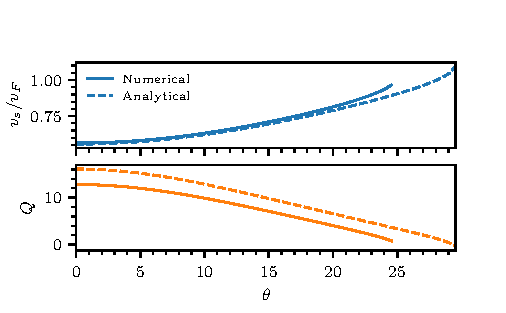
\includegraphics{angles_vs_and_Q}
		\caption{The spin demon velocity (top) and quality factor (bottom), as a function of angle $\theta$. The numerical solutions (solid),  are obtained by numerically finding the zeros and corresponding derivatives from the full dielectric function; the analytical solutions (dashed) follow from numerically solving \cref{eq:zeros-vs}. 
			%			Note that $\eta_{{\mathrm{min}}}/\eta_{{\mathrm{maj}}}=\sqrt{(1+\sigma_{\mathrm{min}}\cos2\theta\, m_0/m_* )/(1+\sigma_{\mathrm{maj}}\cos2\theta\, m_0/m_*)}$.
			\label{fig:vs-and-Q} }
	\end{figure}
	
	\paragraph{Out-of-phase oscillations and magnetic moment. }To gain more insight in the character of the spin demon, we solve the eigenvalue problem defined by \cref{eq:chi-rpa}, 
	\begin{equation}
		\begin{pmatrix}
			\Ree[\chi_{\uparrow}^{(0)}(\omega)]^{-1}-v_q & -v_q \\
			-v_q & \Ree[\chi_{\uparrow}^{(0)}(\omega)]^{-1}-v_q
		\end{pmatrix}\begin{pmatrix}
			\psi_\uparrow \\ \psi_\downarrow
		\end{pmatrix} =0,
	\end{equation}
	which has the solution
	\begin{equation}
		\frac{\psi_{{\mathrm{maj}}}}{\psi_{{\mathrm{min}}}} = -\frac{v_qN_0}{1 + v_qN_0}\approx -1 + O(q^2/\kF^2) \label{eq:out-of-phase},
	\end{equation} 
	where $N_0=\mdos \kF / (2\pi^2\hbar^2)$ is the spin-independent density of states at the Fermi level.
%	Here we stress that  projected majority and minority spin species change as the angle of the spin demon rotates through the altermagnetic plane.
	This result thus clearly shows that in the limit of small $q/\kF$, the spin demon consists of out-of-phase oscillations of two spin-species---in contrast to the conventional plasmon, which consist of in-phase oscillations \cite{agarwalLonglivedSpinPlasmons2014}. \Cref{eq:out-of-phase} also demonstrates that as $q/\kF$ approaches zero, $|{\psi_{{\mathrm{maj}}}}| < |{\psi_{{\mathrm{min}}}}|$. We therefore expect that a spin demon carriers a magnetic moment, since it is composed of predominantly one spin species. 
	
	To show this in more detail, we consider an external magnetic field $B$, with a strength far from the spin-flop transition and which is orientated along the N\'{e}el vector. The electrons then gain energy $\sigma g_e\mu_B B$, with $g_e\approx2$ the electron gyromagnetic ratio and $\mu_B$ the Bohr magneton. We furthermore assume the magnetic field to not affect the magnetic texture, which would be the case in the presence of a (weak) easy-axis anisotropy, and we neglect orbital magnetization effects. We now calculate the magnetic moment, which is defined as
	\begin{equation}
		\mu_d \equiv -\hbar\frac{\partial\omega_d}{\partial B}. \label{eq:mud}
	\end{equation}
	In the limit of $\deltaq\rightarrow0$ we have
	\begin{equation}
		\frac{\partial \vs}{\partial B} = \vs' \frac{\partial\Delta}{\partial B} + O(\Delta^2),
	\end{equation}
	where $\Delta\equiv g_e\mu_B B N'_0 /N_0 $, $ \vs'=8e^{-4}v_F$ and $N'_0=\partial N_0(\epsilon)/\partial\epsilon|_{\epsilon=\epsilon_F}$, 
	This allows us to obtain the magnetic moment as
	\begin{equation}
		\mu_d =  g_e\mu_B\hbar \frac{N'_0}{N_0}  \eta_{\mathrm{min}}(\theta)  \vs' q. \label{eq:mup}
	\end{equation}
	Importantly, a finite magnetic moment implies that a spin demon can carry angular momentum. 
	In addition, since the minority spin species switches between spin-up and spin-down as the spin demon is rotated through the plane, the magnetic moment has the opposite sign for $\bm q \parallel \hat{\bm y}$, representing the $d$-wave symmetry of the underlying altermagnetic band structure. 
	
	\begin{figure}
		\centering
		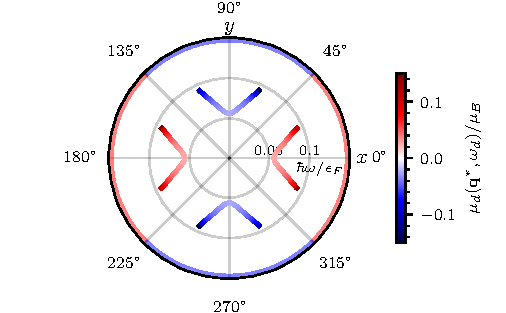
\includegraphics[width=\columnwidth]{polar-plot-sign}
		\caption{Numerically obtained spin demon resonance frequency $\omega_d$ as a function of $\bm q^*=q\ (\cos\theta, \sin\theta,0)$, with $q=0.05\kF$, rotated in the altermagnetic spin splitting plane with angle $\theta$. The color corresponds to the magnetic moment, showing the $d$-wave character. Obtained by numerically finding the zeros and evaluating \cref{eq:mud} from the full dielectric function.
			Along $x$ and $y$, the magnetic moment is approximately $\pm\muB\mu_B$. The colors on the ring indicate the projected spin species. \label{fig:magnetic-moment} }
	\end{figure}
	
	We show this in more detail in \cref{fig:magnetic-moment}, where we have numerically calculated the magnetic moment of the spin demon as a function of $\theta$. For the angles where the spin-up species is the majority species, we obtain a positive magnetic moment, whereas for the angles where the spin-down species is dominant, we have a negative magnetic moment. The magnetic moment thus captures the $d$-wave symmetry of the underlying altermagnetic band structure.
\cref{eq:mup}]. For $q=0.05\kF$, we obtain that $\mu_p\approx\muB\mu_B$ for $\bm q\parallel \xx$. The magnetic moments grows to $\muBmax\mu_B$ for angles approaching the critical angle---but the quality factor also decreases. 
	
	These results show that an applied magnetic field will shift the spin demon frequencies up or down, depending on the orientation of $\bm q$. The shift in the spin demon frequency is however small, approximately \muBShift at $\bm q=0.05k_F\hat{\bm x}$ with a magnetic field of \SI{1}{T}, whereas the energy of the spin demon is \demonenergy, resulting in a relative shift of $\muBShiftrelative\%$. Alternatively, all that is required is a sublattice-sensitive experimental handle, for example achievable through piezomagnetism \cite{aoyamaPiezomagneticPropertiesAltermagnetic2024}.
	
	
	
	
	\paragraph{Two-dimensional. }The spin demon as considered here also exists in two-dimensional altermagnets. The analysis in 2D is similar to in 3D, and we relegate details to Sec.~VIII in the SM. We choose the same parameters as in 3D.
	
	We show the resulting spin-spin response function in \cref{fig:2D}, highlighting the same four-fold rotational symmetry. 
	 In addition, we show the spin demon velocity and quality factor as a function of the projected spin splitting in 2D. Because the particle-hole continuum is sharply defined in two dimensions,  we are able to provide analytical solutions of the spin demon velocity and quality factor as \cite{agarwalLonglivedSpinPlasmons2014}
	\begin{align}
		\vs^{\mathrm{2D}} &= \frac{2}{\sqrt{3}} v_F \eta_{\mathrm{min}}(\theta) q + O(q^2/\kF^2)\\
		Q^{\mathrm{2D}} &= \frac{3\sqrt{4\eta_{\mathrm{min}}^2(\theta)-3\eta_{\mathrm{maj}}^2(\theta)}}{\eta_{\mathrm{min}}(\theta)} + O(q^2/\kF^2),
	\end{align}
	for $2\eta_{\mathrm{min}}(\theta)>\sqrt{3}\eta_{\mathrm{maj}}(\theta)$, whereas the spin demon ceases to exist if this condition is not met. 
	
	
	We observe that the spin demon in two dimensions is more robust than in 3D, surviving for larger $\theta$ ($\criticalangle$ versus $\approx\SI{23}{\degree}$). Beyond this angle we observe the remnants of the overdamped conventional acoustic plasmon. The quality factors are however comparable in magnitude, especially for angles that align with the altermagnetic axis. Finally, we comment that in 2D, the spin demon also has a magnetic moment (shown in Sec.~VIII in the SM), which is comparable in magnitude to the 3D case and displays the same altermagnetic symmetry.
	
	\begin{figure}
		\tikzsetnextfilename{2D}
		\begin{tikzpicture}
			\node at (-0.5\columnwidth,2) {\includegraphics[width=\columnwidth]{2D_polar-plot-chiSzSz}};
			\node at (-0.5\columnwidth,-3) {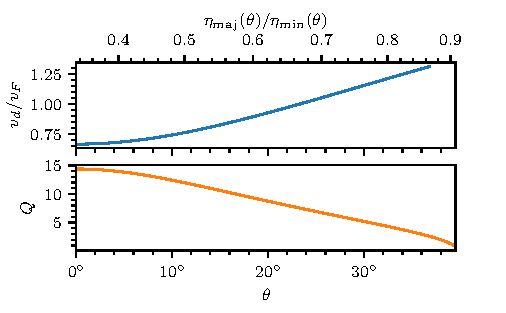
\includegraphics[width=\columnwidth]{2D_angles_vs_and_Q}};
			\node at (-0.8\columnwidth,5) {(a)};
			\node at (-0.8\columnwidth,-0.5) {(b)};
		\end{tikzpicture}
		\caption{In two dimensions: (a) $\Imm[\chi_{S_zS_z}(\bm q^*,\omega)]$, The angle indicates $\theta$ and the radial axis the frequency $\omega$. (b) The spin demon velocity (top) and quality factor (bottom) as a function of rotation angle  $\theta$. \label{fig:2D} }
	\end{figure}
	
	%	We observe that in 2D, the quality factor is bounded and reaches a maximum for $\delta_q=???$ as $Q=???$, which was also observed by \cite{agarwalLonglivedSpinPlasmons2014}. \pg{why?}
	
	
	\paragraph{Conclusion. }We have shown that both three and two dimensional altermagnetic metals can host out-of-phase oscillations of the two spin densities, realizing a spin demon. The spin demon has a magnetic moment, which has opposite sign for propagation along different angles through the altermagnetic plane, inheriting the altermagnetic $d$-wave symmetry.
	
	We have considered here only the RPA, which we expect to provide a fair description, since corrections to the RPA have been shown to mainly enhance the damping of comparable acoustic plasmons in a two-dimensional spin-polarized electron gas \cite{kreilExcitationsSpinpolarizedTwodimensional2015}. We  expect similar conclusions to hold for altermagnetic spin demons.
	
	
	In this work, we have considered a $d$-wave altermagnet, where the spin-split Fermi surfaces are elliptical. We have repeated the same analysis for a $g$-wave altermagnet in Sec.~IX in the SM, where we find that the separation of the spin-polarized particle-hole continua is not sufficient for a spin demon to emerge. We therefore conclude that the spin demon is a specific feature of $d$-wave altermagnets.
%	 which we attribute to the specific form of the long-wavelength dispersion of a $g$-wave altermagnet, which is ill-suited for the emergence of a spin demon.
	

	
	The spin demon could be directly observed by making use of spin-sensitive electron scattering probes, such as spin-polarized electron energy loss spectroscopy (SPEELS) \cite{plihalSpinWaveSignature1999} or cross-polarized Raman scattering \cite{kimPolarizedRamanSpectroscopy2020}. These probes directly measure $\Imm[\chi_{S_zS_z}(\bm q,\omega)]$ (or $\Imm[\chi_{nS_z}(\bm q,\omega)]$, which also contains information of the spin demon; see Sec.~III in the SM), and can thus map \cref{fig:polar} and \subfigref{fig:alongx}{(a)}.
	
	Real samples will most likely consist of multiple magnetic domains with different orientations of the N\'eel vector. We expect that this will not be a difficulty for the detection of the spin demon, since typical domain sizes in altermagnets can be in the micrometer range \cite{aminNanoscaleImagingControl2024a}, placing an upper limit on the spin demon wavelength of micrometers. A probe which is spatially localized on this length scale can then directly detect spin demons. In addition, recent transport experiments have measured a finite anomalous Hall effect signal, demonstrating that altermagnetic domains are not equally populated \cite{jeongMetallicityAnomalousHall2025a,leiviskaAnisotropyAnomalousHall2024, reichlovaObservationSpontaneousAnomalous2024a}, and thus even a spatially delocalized probe could detect spin demons.
	\begin{acknowledgments}
	We thank Khalil Zakeri for insightful discussions. This work is in part funded by the Deutsche Forschungsgemeinschaft (DFG, German Research Foundation) -- Project No.~504261060 (Emmy Noether Programme). P.~G. acknowledges financial support from the Alexander von Humboldt postdoctoral fellowship. 
	\end{acknowledgments}
	\bibliography{spin-plasmons}
\end{document}
